\documentclass[11pt]{beamer}
\usetheme{Madrid}
\usefonttheme{serif}

\usepackage[utf8]{inputenc}
\usepackage[english]{babel}
\usepackage[T1]{fontenc}

\usepackage{amsmath}
\usepackage{amsfonts}
\usepackage{amssymb}
\usepackage{graphicx}

\setbeamertemplate{caption}[numbered]
\setbeamertemplate{navigation symbols}{}

% Author / Title Info
\author[Team]{%
\begin{tabular}{lll}
Goureesh Chandra   & 31 & TVE22CS069 \\
Ivin Mathew Kurian & 33 & TVE22CS075 \\
Muhammed Farhan    & 39 & TVE22CS094 \\
Rethin Francis     & 72 & LTVE22CS149 \\
\end{tabular} \\[8pt]
\textbf{Advisor: Prof. Divya S K}
}

\title{Reinforcement Learning for ICU Treatment Planning}

\institute[]{College of Engineering, Trivandrum \\ Dept. of Computer Science \& Engineering}
\date{\today}

% ---------------------------------------------------------
\begin{document}

% Title
\begin{frame}
  \titlepage
\end{frame}

% Outline of Presentation
\begin{frame}{Outline of Presentation}
  \tableofcontents
\end{frame}

% --------------------------------------
\section{Introduction}
\begin{frame}{Introduction}
Doctors face tough decisions treating critically ill ICU patients with conditions like sepsis. Our AI system learns from ICU data to suggest better plans.

Using reinforcement learning, it builds a "digital twin" simulator to predict patient responses to treatments safely. This enables personalized, safer plans, supporting doctors and reducing risks/costs.
\end{frame}

% --------------------------------------
\section{Problem Statement and Objectives}
\begin{frame}{Problem Statement and Objectives}
\textbf{Problem:} Timely, personalized ICU treatment decisions are challenging due to dynamic conditions and fragmented data.

\begin{itemize}
    \item High-stakes, dynamic trajectories.
    \item Incomplete EHR data.
    \item AI limited to historical mimicry.
\end{itemize}

\textbf{Objectives:}
\begin{itemize}
    \item Build patient simulator from EHR data.
    \item Optimize RL policies safely.
    \item Provide clinical decision support.
\end{itemize}
\end{frame}

% --------------------------------------
\section{Design Methodology and Algorithms}
\begin{frame}{Design Methodology and Algorithms}
This approach is inspired by DreamerV3 and its clinical adaptation in medDreamer.  

\textbf{Two sequential stages:}
\begin{enumerate}
    \item Train the \textbf{Patient Simulator (World Model)} to predict patient outcomes.  
    \item Train the \textbf{RL Agent (Policy)} using the simulator to discover optimal treatments.
\end{enumerate}
\end{frame}

\begin{frame}{Design Methodology and Algorithms: Diagrams}
    \begin{center}
        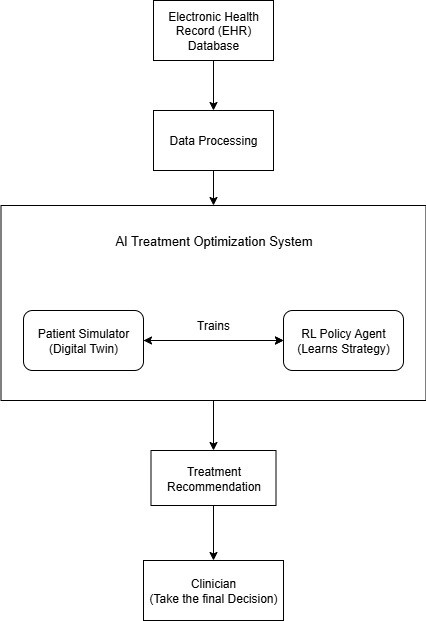
\includegraphics[width=0.45\textwidth]{design_flow.jpg} % Architectural/Flow Diagram
    \end{center}
    \textbf{Key Components:}
    \begin{itemize}
        \item EHR Database (e.g., MIMIC-IV)
        \item Data Preprocessing
        \item Patient Simulator (Digital Twin)
        \item RL Policy Agent
        \item Treatment Recommendation
    \end{itemize}
\end{frame}

\begin{frame}{Algorithm 1: Patient Simulator Training}
\textbf{Goal:} Learn patient health dynamics from EHR data to create a reliable "digital twin".  

\textbf{Steps:}
\begin{enumerate}
    \item \textbf{Initialization:} Neural network parameters $\phi$  
    \begin{itemize}
        \item Encoder
        \item Dynamics predictor
        \item Prediction heads (reconstruction, rewards, outcomes)
    \end{itemize}
    \item \textbf{Training Loop:} For multiple epochs:
    \begin{enumerate}
        \item Sample patient trajectories (observations, actions, rewards)
        \item Encode observations to latent states $s_t$
        \item Predict next latent state $s_{t+1}$ given $s_t$ and action $a_t$
        \item Reconstruct observations and predict rewards/outcomes
        \item Compute combined loss and update $\phi$ via backpropagation
    \end{enumerate}
    \item \textbf{Output:} Trained Patient Simulator for realistic patient trajectories
\end{enumerate}
\end{frame}

\begin{frame}{Algorithm 2: RL Agent Training}
\textbf{Goal:} Train an optimal treatment policy safely in the simulated environment.

\textbf{Steps:}
\begin{enumerate}
    \item Load trained Patient Simulator (weights frozen)
    \item Initialize RL Agent: policy network $\theta$ (actor), value network $\psi$ (critic)
\end{enumerate}

\textbf{Phase 1: Clinically Grounded Policy Initialization}  
\begin{itemize}
    \item Generate hybrid trajectories (real data + short simulator rollouts)
    \item Train actor and critic:
    \begin{itemize}
        \item Critic: evaluate long-term state values
        \item Actor: choose actions leading to high-value states
    \end{itemize}
\end{itemize}
\end{frame}

\begin{frame}{Algorithm 2 (cont.): Strategic Refinement}
\textbf{Phase 2: Strategic Refinement through Long-Horizon Imagination}  
\begin{itemize}
    \item Generate fully imagined trajectories using the Patient Simulator
    \item Fine-tune actor and critic to improve long-term planning
\end{itemize}

\textbf{Output:} Final trained \textbf{Optimal Treatment Policy} that recommends actions given a patient’s current state
\end{frame}

% --------------------------------------
\section{Implementation Setup Framework}
\begin{frame}{Implementation Setup Framework}
\textbf{4.1 Hardware and Software Requirements}  
\begin{itemize}
    \item \textbf{Hardware:} GPU-enabled system (RTX 4060/4090 or cloud GPUs).
    \item \textbf{Software:} Python, PyTorch, Ray RLlib, pandas, NumPy, scikit-learn.
\end{itemize}

\textbf{4.2 Implementation Environment Setup}  
\begin{itemize}
    \item Datasets: MIMIC-III, MIMIC-IV, eICU.
    \item Preprocessing: Clean and structure EHR data into trajectories.
    \item Frameworks: PyTorch for neural networks, Ray RLlib for RL.
\end{itemize}
\end{frame}

% --------------------------------------
\section{Implementation Results}
\begin{frame}{Implementation Results}
\textbf{Phase-1 Results:} As this is Phase-1, full implementation is ongoing. Preliminary results include:
\begin{itemize}
    \item Data preprocessing completed for MIMIC-IV demo.
    \item Patient Simulator training initiated (e.g., loss curves placeholder).
    \item Synthetic FHIR Bundle generation for data validation.
\end{itemize}

\textbf{Graphs/Tables:} 
\begin{itemize}
    \item Example: Training loss over epochs (insert graph if available).
    \item Screenshots: Model architecture diagram.
\end{itemize}
% Note: Insert actual graphs/tables/screenshots here for visibility.
\end{frame}

% --------------------------------------
\section{Individual Contributions}
\begin{frame}{Individual Contributions}
\begin{itemize}
    \item \textbf{Goureesh Chandra (TVE22CS069):} Literature review, algorithm design, and data preprocessing.
    \item \textbf{Ivin Mathew Kurian (TVE22CS075):} Model implementation, simulator training, and notebook development.
    \item \textbf{Muhammed Farhan (TVE22CS094):} RL agent training, evaluation, and presentation preparation.
    \item \textbf{Rethin Francis (LTVE22CS149):} Data handling, FHIR mapping, and documentation.
\end{itemize}
\end{frame}

% --------------------------------------
\section{Future Works (Project Phase-2)}
\begin{frame}{Future Works (Project Phase-2)}
\begin{itemize}
    \item Complete full RL training and evaluation on larger datasets.
    \item Extend framework to other diseases (e.g., diabetes, cancer care).  
    \item Incorporate multi-modal data (genomics, imaging).  
    \item Clinician-in-the-loop evaluation and real-world validation.
\end{itemize}
\end{frame}

% --------------------------------------
\section{Conclusion}
\begin{frame}{Conclusion}
\begin{itemize}
    \item We are developing a \textbf{model-based reinforcement learning framework} trained on ICU data for clinical decision support.  
    \vspace{6pt}
    \item By building a \textbf{digital twin of patients}, the system safely explores treatment strategies without direct risk to patients.  
    \vspace{6pt}
    \item The approach enables \textbf{personalized and safer treatment recommendations}, reducing unnecessary interventions and improving patient outcomes.  
    \vspace{6pt}
    \item Future work includes extending the model to more diverse patient populations and validating in real-world clinical settings.  
\end{itemize}
\end{frame}

% --------------------------------------
\section{References}
\begin{frame}{References}
\tiny
\begin{thebibliography}{9}

\bibitem{xu2025}
Qianyi Xu, Dilruk Perera, Gousia Habib, and Mengling Feng (2025).
\newblock medDreamer: Model-Based Reinforcement Learning with Latent Imagination on Complex EHRs for Clinical Decision Support.
\newblock \textit{arXiv preprint arXiv:2505.19785}.

\bibitem{komorowski2021}
Arthur Komorowski et al. (2021).
\newblock Challenges with reinforcement learning model transportability for sepsis treatment in emergency care.
\newblock \textit{Critical Care Medicine}.

\bibitem{amirahmadi2023}
Ali Amirahmadi, Mattias Ohlsson, and Kobra Etminani (2023).
\newblock Deep learning prediction models based on EHR trajectories: A systematic review.
\newblock \textit{Journal of Biomedical Informatics}.

\bibitem{nambiar2023}
Mila Nambiar et al. (2023).
\newblock Deep offline reinforcement learning for real-world treatment optimization applications.
\newblock \textit{arXiv preprint arXiv:2302.07549}.


\bibitem{r2i2023}
Anon. Authors (2023).
\newblock Mastering Memory Tasks with World Models.
\newblock \textit{ICML}.

\bibitem{debrouwer2022}
Edward De Brouwer, Javier González Hernández, and Stephanie Hyland (2022).
\newblock Predicting the impact of treatments over time with uncertainty aware neural differential equations.
\newblock \textit{AISTATS}.

\bibitem{kondrup2023}
Flemming Kondrup et al. (2023).
\newblock Towards Safe Mechanical Ventilation Treatment Using Deep Offline Reinforcement Learning.
\newblock \textit{AAAI-23}.

\end{thebibliography}
\end{frame}


% --------------------------------------
\begin{frame}
\begin{center}
    \Huge{Thank You!}
\end{center}
\end{frame}

\end{document}
\end{frame}

\end{document}
    \vspace{0.3cm}
    \textbf{5. Clinician (Final Decision)}
    \begin{itemize}
        \item Doctor reviews AI suggestions
        \item Combines with expertise, ethics, patient context
        \item Ensures safety and accountability
    \end{itemize}
\end{frame}

% --------------------------------------
\section{Resource Allocation}
\begin{frame}{Resource Allocation}
\textbf{1. Data Resources}  
\begin{itemize}
    \item MIMIC-III, MIMIC-IV, eICU datasets.
    \item Preprocessing: Python (pandas, NumPy, scikit-learn).
\end{itemize}

\textbf{2. Computational Resources}  
\begin{itemize}
    \item GPU-enabled system (RTX 4060/4090 or cloud GPUs).
    \item Frameworks: PyTorch, Ray RLlib.
\end{itemize}
\end{frame}



% --------------------------------------
\section{Future Work}
\begin{frame}{Future Work}
\begin{itemize}
    \item Extend framework to other diseases (e.g., diabetes, cancer care).  
    \item Incorporate multi-modal data (genomics, imaging).  
    \item Clinician-in-the-loop evaluation.  
\end{itemize}
\end{frame}


% --------------------------------------
\section{Conclusion}
\begin{frame}{Conclusion}
\begin{itemize}
    \item We are developing a \textbf{model-based reinforcement learning framework} trained on ICU data for clinical decision support.  
    \vspace{6pt}
    \item By building a \textbf{digital twin of patients}, the system safely explores treatment strategies without direct risk to patients.  
    \vspace{6pt}
    \item The approach enables \textbf{personalized and safer treatment recommendations}, reducing unnecessary interventions and improving patient outcomes.  
    \vspace{6pt}
    \item Future work includes extending the model to more diverse patient populations and validating in real-world clinical settings.  
\end{itemize}
\end{frame}



% --------------------------------------
\section{References}
\begin{frame}{References}
\tiny
\begin{thebibliography}{9}

\bibitem{xu2025}
Qianyi Xu, Dilruk Perera, Gousia Habib, and Mengling Feng (2025).
\newblock medDreamer: Model-Based Reinforcement Learning with Latent Imagination on Complex EHRs for Clinical Decision Support.
\newblock \textit{arXiv preprint arXiv:2505.19785}.

\bibitem{komorowski2021}
Arthur Komorowski et al. (2021).
\newblock Challenges with reinforcement learning model transportability for sepsis treatment in emergency care.
\newblock \textit{Critical Care Medicine}.

\bibitem{amirahmadi2023}
Ali Amirahmadi, Mattias Ohlsson, and Kobra Etminani (2023).
\newblock Deep learning prediction models based on EHR trajectories: A systematic review.
\newblock \textit{Journal of Biomedical Informatics}.

\bibitem{nambiar2023}
Mila Nambiar et al. (2023).
\newblock Deep offline reinforcement learning for real-world treatment optimization applications.
\newblock \textit{arXiv preprint arXiv:2302.07549}.


\bibitem{r2i2023}
Anon. Authors (2023).
\newblock Mastering Memory Tasks with World Models.
\newblock \textit{ICML}.

\bibitem{debrouwer2022}
Edward De Brouwer, Javier González Hernández, and Stephanie Hyland (2022).
\newblock Predicting the impact of treatments over time with uncertainty aware neural differential equations.
\newblock \textit{AISTATS}.

\bibitem{kondrup2023}
Flemming Kondrup et al. (2023).
\newblock Towards Safe Mechanical Ventilation Treatment Using Deep Offline Reinforcement Learning.
\newblock \textit{AAAI-23}.

\end{thebibliography}
\end{frame}


% --------------------------------------
\begin{frame}
\begin{center}
    \Huge{Thank You!}
\end{center}
\end{frame}

\end{document}
